%-----------------------------------------------------------------------------
%
%               Template for sigplanconf LaTeX Class
%
% Name:         sigplanconf-template.tex
%
% Purpose:      A template for sigplanconf.cls, which is a LaTeX 2e class
%               file for SIGPLAN conference proceedings.
%
% Guide:        Refer to "Author's Guide to the ACM SIGPLAN Class,"
%               sigplanconf-guide.pdf
%
% Author:       Paul C. Anagnostopoulos
%               Windfall Software
%               978 371-2316
%               paul@windfall.com
%
% Created:      15 February 2005
%
%-----------------------------------------------------------------------------


\documentclass[10pt,numbers,preprint,nocopyrightspace]{sigplanconf}

% The following \documentclass options may be useful:

% preprint      Remove this option only once the paper is in final form.
% 10pt          To set in 10-point type instead of 9-point.
% 11pt          To set in 11-point type instead of 9-point.
% numbers       To obtain numeric citation style instead of author/year.

\newif\iffull
\fullfalse

\usepackage{times}
\usepackage{graphicx}
\usepackage{mathtools}
\usepackage{amsmath}
\usepackage[utf8]{inputenc}
\usepackage{cleveref}
\usepackage{listings}
\usepackage{array}
\usepackage{breqn}
\usepackage{tikz}
\usepackage{algorithmicx}
\usepackage[Algorithm,ruled]{algorithm}
\usepackage{algpseudocode}
\usepackage{pifont,xspace}
\usetikzlibrary{automata,positioning,shapes.geometric}
\newcommand{\name}{Zeppelin\xspace}
\newcommand{\Name}{\name}
\newcommand{\genesis}{Genesis\xspace}
\newcommand{\pushcode}[1][1]{\hskip\dimexpr#1\algorithmicindent\relax}
\newcolumntype{P}[1]{>{\centering\arraybackslash}p{#1}}

\usepackage[font=small]{caption}
\usepackage{enumitem}
%\usepackage{usenix}
\usepackage{epsfig}
%\usepackage[TABBOTCAP]{subfigure}
\usepackage{color}
%\usepackage{thumbpdf}
\usepackage{verbatim}
%\usepackage{hyperref}
\usepackage{url}
%\usepackage{booktabs}
\usepackage{colortbl}
\usepackage{enumitem}
\usepackage[export]{adjustbox}
\usepackage{subfig}
\usepackage{mathtools}
\usepackage{amsthm}
\usepackage{multirow}% http://ctan.org/pkg/multirow
\usepackage{hhline}
\newcommand{\minisection}[1]{\smallskip\noindent{\bf #1.}}
\newcommand{\secref}[1]{{\S\ref{#1}}}
\newcommand{\secsref}[2]{{Sections~\ref{#1} and \S\ref{#2}}}
\newcommand{\figref}[1]{{Figure~\ref{#1}}}
\newcommand{\figsref}[2]{{Figure~\ref{#1} and \ref{#2}}}
\newcommand{\appref}[1]{{Appendix~\ref{#1}}}
\newcommand{\thmref}[1]{{Theorem~\ref{#1}}}
\newcommand{\lemref}[1]{{Lemma~\ref{#1}}}
\newcommand{\corref}[1]{{Corollary~\ref{#1}}}
\newcommand{\proref}[1]{{Property~\ref{#1}}}
\newcommand{\tabref}[1]{{Table~\ref{#1}}}


\newcommand{\compactcaption}[1]{\vspace{-1em}\caption{#1}\vspace{-1em}}
\newcommand{\botcompactcaption}[1]{\caption{#1}\vspace{-1em}}
\newcommand{\topcompactcaption}[1]{\vspace{-1em}\caption{#1}\vspace{-0.5em}}

\newenvironment{compactitemize}
{
   \begin{itemize}[leftmargin=1.5em]
   \vspace{-1ex}
   \setlength{\topsep}{0pt}
   \setlength{\itemsep}{0em}
   \setlength{\parskip}{0pt}
   \setlength{\parsep}{0pt}
}
{
   \vspace{-1ex}
   \end{itemize}
}
\newenvironment{compact2itemize}
{
	\begin{itemize}[leftmargin=1.5em]
		\vspace{-1ex}
		\setlength{\topsep}{0pt}
		\setlength{\itemsep}{0.5em}
		\setlength{\parskip}{0pt}
		\setlength{\parsep}{0pt}
	}
	{
		\vspace{-1ex}
	\end{itemize}
}


\newenvironment{compactenumerate}
{
   \begin{enumerate}[leftmargin=1.5em]
   \vspace{-1ex}
   \setlength{\topsep}{0pt}
   \setlength{\itemsep}{0em}
   \setlength{\parskip}{0pt}
   \setlength{\parsep}{0pt}
}
{
   \vspace{-1ex}
   \end{enumerate}
}

%\usepackage[small,compact]{titlesec}
%\usepackage[font={bf,small}]{caption}
\usepackage{titlesec}
%\titlespacing*{\section}{1pt}{3pt}{3pt}
%\titlespacing*{\subsection}{1pt}{3pt}{1.5pt}
%\titlespacing*{\subsubsection}{1pt}{3pt}{2pt}
\newtheorem{example}{Example}
\newtheorem{theorem}{Theorem}[section]
\newtheorem{lemma}{Lemma}[section]
\lstset{
	basicstyle=\itshape,
	xleftmargin=2em,
	literate={->}{$\rightarrow$}{2}
	{α}{$\alpha$}{1}
	{δ}{$\delta$}{1}
}

\crefname{Section}{§}{§§}
\Crefname{Section}{§}{§§}


\usepackage{color}
\newcommand{\loris}[1]{\textcolor[rgb]{0.00,0.00,1.00}{L: #1}}
\newcommand{\aditya}[1]{\textcolor[rgb]{0.00,0.00,1.00}{A:#1}}
\newcommand{\kausik}[1]{\textcolor[rgb]{0.00,1.00,0.00}{K: #1}}
\newcommand{\todo}[1]{{\color{red}{\bf TODO: #1}}}

\usepackage{float}

\newcommand{\cL}{{\cal L}}

\begin{document}

%\special{papersize=8.5in,11in}
%\setlength{\pdfpageheight}{\paperheight}
%\setlength{\pdfpagewidth}{\paperwidth}
%
%\conferenceinfo{CONF 'yy}{Month d--d, 20yy, City, ST, Country}
%\copyrightyear{20yy}
%\copyrightdata{978-1-nnnn-nnnn-n/yy/mm}
%\copyrightdoi{nnnnnnn.nnnnnnn}

% Uncomment the publication rights you want to use.
%\publicationrights{transferred}
%\publicationrights{licensed}     % this is the default
%\publicationrights{author-pays}

%\titlebanner{}        % These are ignored unless
%\preprintfooter{}   % 'preprint' option specified.

\title{Router Configuration Synthesis from Intents}

\authorinfo{Omitted for double blind}
{...}
{...}

\maketitle

\section{Introduction}

Network operators of enterprise and cloud datacenter networks deal
with thousands of flow groups traversing large number of heterogeneous
devices. With growing diversity of applications, need for security and
compliance, and the advent of cloud comouting, these flow groups may
be subject to increasingly complex policies. Cloud tenants or
enterprises require basic reachability between hosts/application, and
middlebox traversal for certain flow groups. Operators, on top of that
require support for policies like traffic isolation between flows to
provide security and fairness, and satisfying resource constraints
pertaining link bandwidths and switch table sizes to perform traffic
engineering and network resource management.  However, configuring
network devices to implement these diverse and complex policies is
manual, ad-hoc and error prone today, leading to violations of
service-level agreements and mis-configurations which have severe
performance and security impacts.

%%  However, in real-life, the
%% process of policy enforcement by network operators is manual and
%% ad-hoc, leading to violations of service-level agreements and
%% mis-configurations which have severe performance and security
%% impacts. With the boom in cloud services, datacenter networks deal
%% with thousands of flows which are not constant, but in flux, thus,
%% making it difficult to enforce them in an ad-hoc manner.

%% Network operators desire various different end-to-end policies to
%% support in clouds and enterprise networks. Tenants or organisations
%% require support for basic policies like reachability between hosts,
%% and specifying different middlebox policies for certain
%% flows. Operators, on top of that require support for complex policies
%% like traffic isolation between flows to provide fairness and
%% specifying resource constraints like link bandwidth and switch table
%% sizes to perform traffic engineering and network resource management.

Though Software-defined Networking (SDN) has allowed network operators
to program networks in a more intuitive manner, many of existing SDN
tools/frameworks are too low-level in their functionality. Supporting
the aforementioned types of policies simply using SDN-capable switches
or with existing languages like Frenetic~\cite{frenetic} and
Pyretic~\cite{pyretic} is extremely challenging; operators would
ideally want to specify and realize policies network-wide without
programming individual switch behaviors. \aditya{we need to be careful
  not to bin all SDN languages into this switch-by-switch model}.
There has been research in the field of network-wide policy
enforcement in networks, like bandwidth provisioning in Merlin
\cite{Merlin}, and middlebox policy enforcement in SIMPLE
\cite{simple} or FlowTags~\cite{flowtags}. However, these approaches
are tailor-made to specific policies, and thus, difficult to extend it
to support other kinds of policies.

In this paper, we seek a {\em general} approach, where operators can
specify a variety of custom policies in a simple, declarative way, and
the complexities of correctly realizing the policies in the data plane
are hidden away from them. %% To support a cornucopia of policies, an
%% important feature is \emph{generality} of the approach of policy
%% enforcement, so that it can be extended to enforce custom policies
%% required by the operator.
By designing and implementing a system called \Name, this paper makes
a case for using \emph{efficient synthesis} of switch table forward
rules to realize this vision.
%% switch
%% table forwarding rules to the solve the problem of policy enforcement
%% by use of off-the-shelf SMT-solvers.

We show that enforcement of several of the policies supported by
\Name, specifically isolation, and middlebox traversal is
NP-complete. Thus, \Name leverages recent advances in creating fast
SMT solvers (e.g., Z3~\cite{z3}) to perform synthesis by encoding the
policy enforcement problem to a SMT instance, and using the SMT solver
to search for a solution, which is then translated into switch
rules. %% This paper presents Genesis, a
%% network management tool where the network operators can express the
%% network-wide policies in a high-level declarative manner and Genesis
%% will synthesize the lower-level switch forwarding rules for realising
%% these policies, eliminating the need for operators to work on
%% switch-level behaviours.
By leveraging a formal reasoning technique of SAT/SMT solving, \Name
eliminates the room for error in policy enforcement.

Unfortunately, naive application of SMT solvers results in synthesis
speeds that don't match the scale of operations of cloud and
enterprise networks today. \aditya{give an example as to how slow
  things can get} To overcome this challenge, \Name leverages a few
domain-specific ideas.  Specifically, it uses a novel search strategy
using regular expressions to prune the space of forwarding plane
configurations by leveraging data center network
structure. \aditya{the previous sentence is vague} knowlegde. Second,
\Name uses heuristical synthesis routine that leverages the nature of
policy interactions to improve synthesis performance. \aditya{quickly
  talk about in 1-2 sentences the speedup achieved with these
  optimizations}

%% are
%% huge, and by supporting a set of diverse and complex policies with
%% different search objectives, we require to create a model general and
%% expressive enough to support these. This poses a challenge as to can
%% synthesis performance be improved by leveraging knowledge specific to
%% the problem of policy enforcement in networks?

We implement \Name using ... We evaluate it using .... Key highlights .... \aditya{all of these are todo}.

Thus, the main contribution of this paper are: \aditya{todo}

%% : We present the design and implementation of a network management
%% system with support for a diverse set of complex end-to-end
%% policies like isolation, waypoints and capacity. We designed a
%% novel search strategy using regular expressions to prune the space
%% of forwarding plane configurations by leveraging the network
%% structure to provide properties of the path, especially in
%% datacenter topologies. Lastly, we design a heuristical synthesis
%% routine leveraging the nature of policy interactions to improve
%% synthesis performance.

\section{Motivation} \label{sec:motivation}
% Programming a legacy network control plane to satisfy a variety of
% connectivity, security, and performance policies is a complex and error-prone
% task. We have shown that program synthesis is a promising approach to automate
% this process and produce a control plane that is ``correct-by-construction.''
% In particular, we presented an architecture where a network operator provides
% a policy-compliant data plane and a set of hard and soft policies as input,
% and the system automatically provides a set of device configurations that
% leverage the control plane features available on each device to compute
% policy-compliant paths, even in the presence of failures.  Formulating a
% tractable synthesis problem and maximizing the number of satisfied soft
% policies are the key challenges in realizing this vision. We show these
% challenges can be overcome by modeling the control plane using a graph-based 
% abstract representation tied to a traditional shortest path algorithm and
% iteratively transforming the abstract representation based on feedback from
% the satisfiability (SAT) solver and characteristics of the graph. However, we
% have only explored how to address a subset of important policies and leverage a
% few available control plane features on traditional networking hardware. Our
% future work will focus on satisfying a wider range of policies using more
% features, and we will study how to best translate our abstract representation
% into actual device configurations to make our system practical for use with
% real networks.

One of the foremost tasks in network management is programming the network to
forward traffic in a manner consistent with user- and application-induced
policies. Common types of policies include: reachability (i.e., which
end-hosts can communicate), isolation (i.e., which flows cannot share links),
service chaining (i.e., which middleboxes must be traversed), resilience
(e.g., how many backup paths are available), and traffic engineering 
objectives like minimizing the average link utilization. Every
set of forwarding paths (i.e., data plane) installed in the network
%---either manually or by a control plane---
should conform to these 
policies, otherwise performance, security, or availability problems may arise.

% A variety of techniques can be used to determine the appropriate forwarding
% paths. One option is to compute a data plane offline, and install the data
% plane using an API that allows direct control of switches' forwarding tables
% (e.g., OpenFlow). Several recent works~\cite{merlin} have adopted this
% approach, using solvers to automatically compute a data
% plane that conforms to a set of policies. 
% A second option is to dynamically compute forwarding
% paths at a logically centralized controller---i.e., use a software-defined
% networking (SDN) control plane. However, this requires developing algorithms
% that take the set of policies and the current state of the network (e.g.,
% which links have failed) as input and output paths that conform to a
% multiplicity of policies.  Most existing SDN control applications only compute
% paths based on one or a few types of policies: e.g., service
% chaining~\cite{simple, flowtags}, traffic engineering~\cite{swan, b4}, or
% resilience~\cite{plinko}. Furthermore, in both approaches, the centralized policy
% component may become bottlenecked
% or fail (even if it is distributed), leading to (a partial) network failure.

A common theme among these policies is that 
they specify \emph{network-wide intent}~\cite{intent},
operators can specify what they \emph{want} from the network as a 
whole, instead of \emph{how} individual components of the network
must be configured. 
Software-defined networking (SDN) has led to the development 
of various frameworks for network-wide policy enforcement
~\cite{netkat, simple, merlin, fattire, genesis}. In SDN,
a centralized controller machine (control plane) controls
the end-to-end paths by managing forwarding rules on programmable
network switches (data plane). The controller can program
forwarding rules using the global view of the network
topology to meet application requirements. While SDN 
significantly enhances programmability of the network to 
satisfy the diverse policy requirements in multi-tenant
clouds and enterprise networks, it suffers from two 
major challenges: 
\emph{scalability} and \emph{failure-tolerance}. 

The centralized controller is responsible for installing 
forwarding rules to all switches, and thus, as network sizes
increase, the overhead of rule installation could increase
significantly. When a network failure (link/switch) occurs,
the controller has to detect and respond to the failure, and
even establishing connectivity between endpoints could be delayed.
Also, the controller is a central point of failure and controller
failure can lead to network disruptions. 
The principles of scalability and failure-tolerance 
were instrumental to the design
of 'traditional' networks (e.g., the Internet) using distributed
routing protocols like OSPF and BGP to manage forwarding in the 
network without a central control entity. Another reason for the 
slow adoption of SDN has been the cost involved in overhaul 
of the network with programmable switches.  

Unlike SDN which provide a clean abstraction
to program the network to satisfy policies 
on end-to-end paths,
programming (i.e., configuring) 
routers such that the paths computed by
the distributed routing protocols enforce the 
policies is challenging for several reasons: 
\setlist[itemize]{
    topsep=.5ex,
    itemsep=0ex,
    leftmargin=1em,
}
\begin{itemize}
%\setlength{\topsep}{0ex}
%\setlength{\itemsep}{0ex}
%\setlength{\parskip}{0pt}
%\setlength{\parsep}{0pt}
\item The available path-computation algorithms
available are predefined---e.g., OSPF uses
Dijkstra's shortest path---and their behavior can only be influenced
through a limited set of parameters---e.g.,
link weights. Similarly, BGP uses shortest
path routing at a domain-granularity, and have different
provisions to control routing (like local preferences).  
\item Operators can have 
heteregeneous protocol requirements based on operational
factors like scalability and cost, thus requiring to model
protocol interactions. 
\item Most policies are
global---i.e., they concern end-to-end paths, not individual devices and
links---making it difficult to map policies to
individual router configurations. 
\item Since failure-tolerance is handled in a distributed 
fashion with no involvement of a central control entity,  
failure-tolerance properties like resilience under bounded
number of network failures must be taken into account in
the generation of router configurations. 

%A single set of parameters must result in
%policy-compliant paths under all reasonable network states---e.g., a bounded
%number of link failures.
\end{itemize}

\begin{figure}
\centering
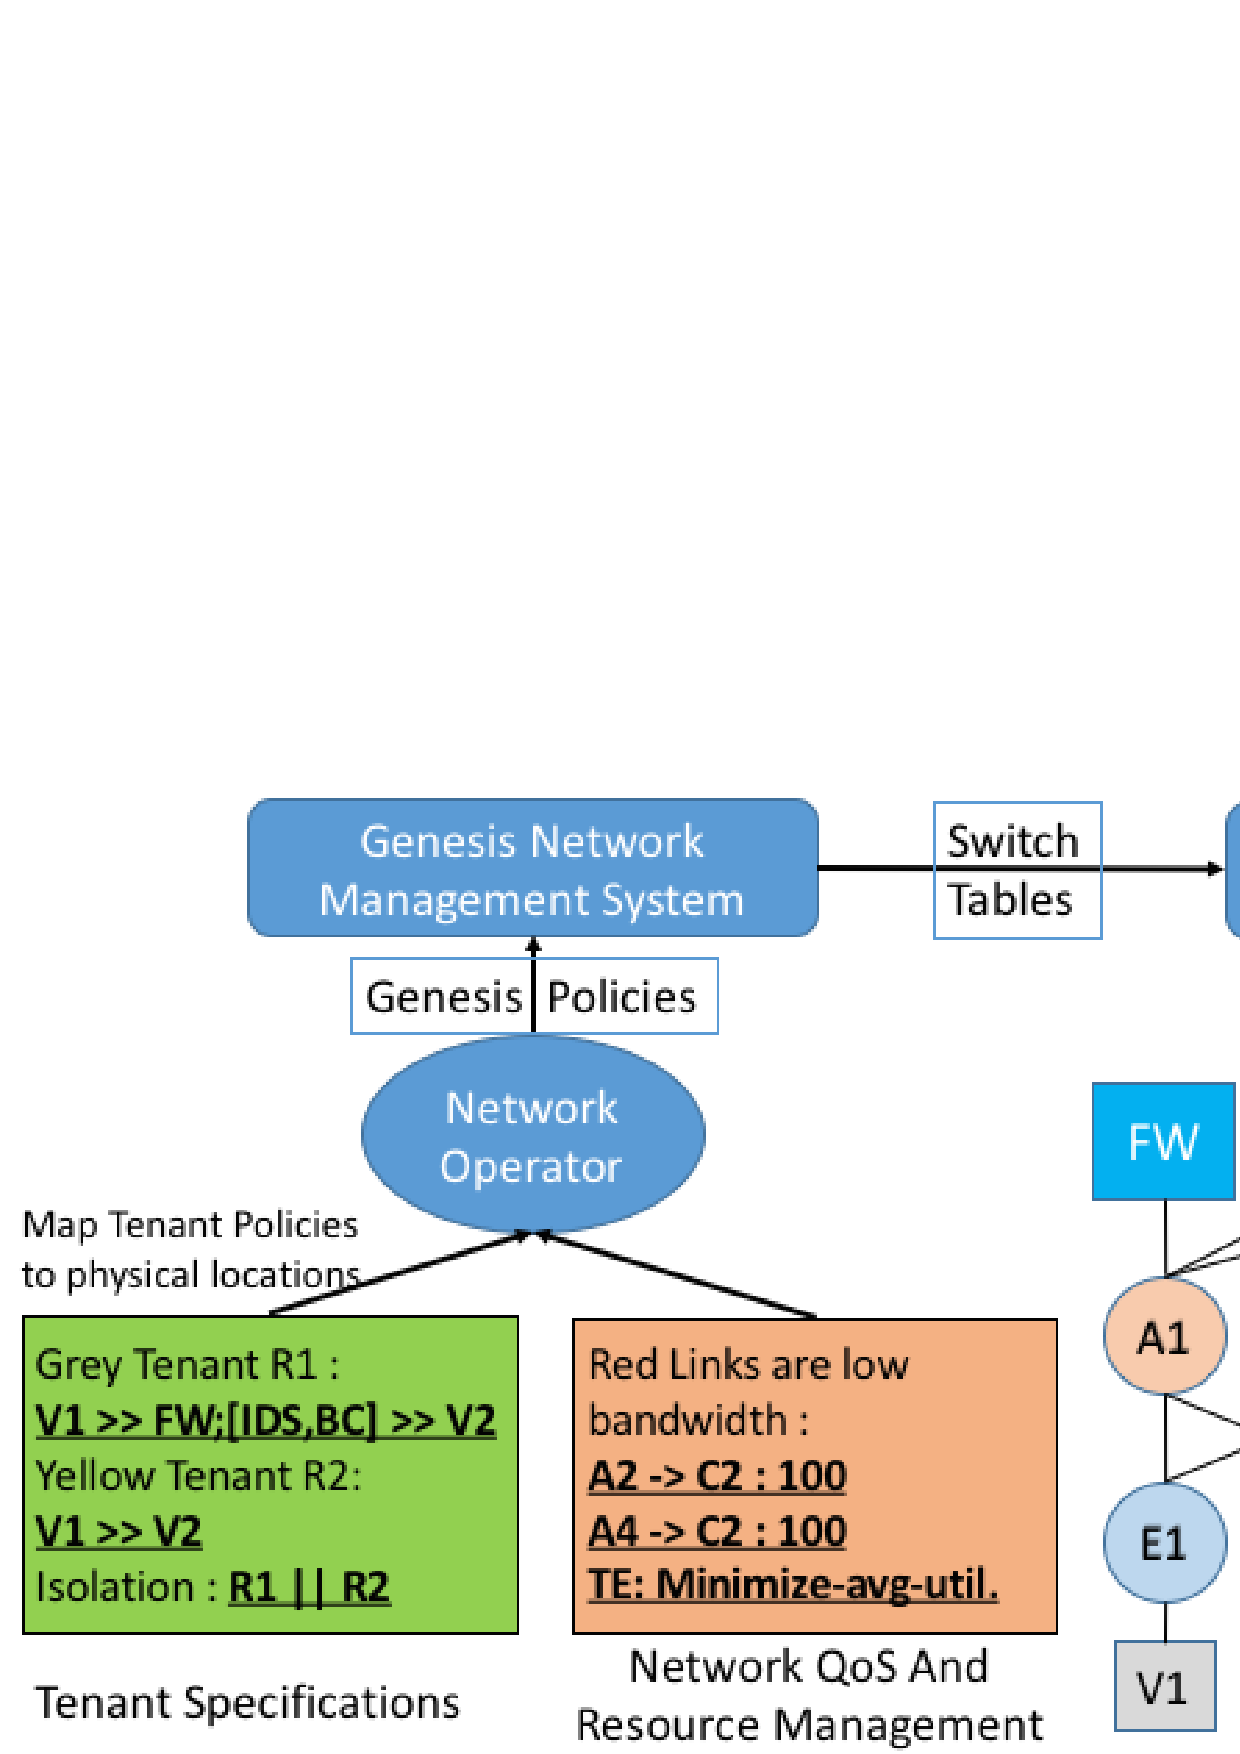
\includegraphics[width=\columnwidth]{figures/architecture.pdf}
\compactcaption{Two-phase process for generating a control plane
       with failure-tolerance properties}
\label{fig:architecture}
\end{figure}

\minisection{Configuration Synthesis}
To address the following challenges, we propose
\emph{automatic synthesis} of configurations, such that 
the network forwarding behaviour of the distributed
control plane meets policy specifications. 
Unfortunately, this task is inherently challenging 
as it requires solving in one shot multiple
computationally hard problems.
For example, even when considering 
static routing and no failures, 
synthesizing configurations 
that satisfy policies 
such as isolation and waypoints
is an NP-hard problem~\cite{genesis}.
Although the progress in SMT solving 
has made many NP-hard problems more practical, 
attempts of incorporating concepts such 
as shortest path algorithms 
into these solvers have resulted 
into huge performance losses~\cite{monosat}, 
not suited for real-world networks.

Our proposed approach is to tackle these problems 
in separate phases
(\figref{fig:architecture}).
First we synthesize a data plane that 
meets the input policies (\secref{sec:genesis}).
Using the data plane as input 
to the second phase, we 
express the problem of 
finding router configurations which 
induce the data plane provided by the
first phase using distributed routing
protocols (OSPF, BGP). Our contribution 
is \name, a framework for synthesizing
router configurations from the data
plane (paths) as input. 

\minisection{OSPF Synthesis}
For the OSPF protocol, configurations assign
weights to links between routers (directed edges
in the network topology). When the network has
to forward a packet from $s$ to $t$, the
OSPF routers uses 
Djikstra's algorithm to chose the
shortest weighted path from $s$ to $t$. Thus,
given input paths, \name finds edge weights 
(which are global for all paths) such that 
the shortest path through the network
for these endpoints exactly match the input paths. 
For example in \Cref{fig:ospfexample}(a), if the input
path is $s\rightarrow r_1 \rightarrow t$ for
destination IP $\lambda$, \name assigns
edge weights such that the input path has a strictly
smaller weight ($w=1+2$) than the other path $s \rightarrow t$ 
($w=5$). Thus, the OSPF routers will forward traffic for
$\lambda$ from $s$ to $t$ through $r_1$. \name 
efficiently computes weights by generating constraints
in the theory of Linear rational arithmetic (LRA) and
uses fast off-the-shelf LP Solvers 
(\secref{sec:ospfsynthesis}). 

However, given a set of paths as input, there may
not exist a solution to the edge weights. Consider the 
input paths as shown in \Cref{fig:ospfexample}(b). 
Both the red and blue paths are required 
to be the unique shortest path between $s$ to $t$
and, clearly, this is cannot be enforced for any 
choice of the edge weights (as weights correspond 
to all destinations). 
One way to synthesize configurations in this scenario 
is to ``disable'' the edge
$(s, t)$ for destination $\lambda_1$.
Using this technique, 
there is only one possible path from $s$ to $t$
for destination $\lambda_1$ ($s\rightarrow r_1 \rightarrow t$),
therefore is chosen as the shortest path. For 
destination $\lambda_2$, the $s\rightarrow t$ path
has a smaller weight ($w=1$) than the
$s\rightarrow r_1 \rightarrow t$ path ($w=1+2$), therefore,
both traffic is forwarded through the input paths for
both the destinations. 
This blocking mechanism is called a route-filter, and
we modify \name's OSPF synthesis algorithm to support
route-filtering (\secref{sec:filtering}).
 

\begin{figure}
	\centering
	\subfloat[Edge Weights]{
		\raisebox{0.5cm}{\resizebox {0.5\columnwidth} {!} {
	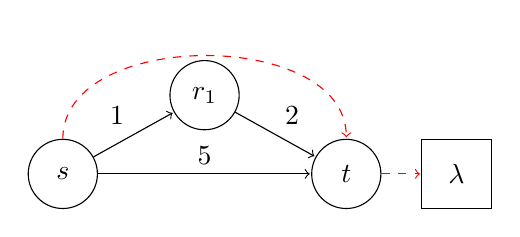
\begin{tikzpicture}[shorten >=0.5pt,node distance=,on grid,auto,
	square/.style={regular polygon,regular polygon sides=4}] 
	\node[state] at (0,0) (s)  {$s$}; 
	\node[state] at (1.8,1) (v1)  {$r_1$}; 
	\node[state] at (3.6, 0)(t) {$t$};
	\node[state, rectangle] at (5, 0) (d1) {$\lambda$};
	\path[->] 
	(s) edge node {1} (v1)
	edge  node {5} (t)
	edge [red, dashed, bend left=90] node {} (t)
	(v1) edge node {2} (t)
	(t) edge [red, dashed] node {} (d1);
	\end{tikzpicture}
	}}}
	\subfloat[Route-Filters]{
			\resizebox {0.5\columnwidth} {!} {
		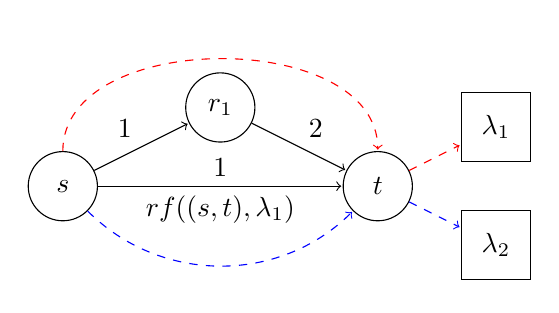
\begin{tikzpicture}[shorten >=0.5pt,node distance=,on grid,auto,
		square/.style={regular polygon,regular polygon sides=4}] 
		\node[state] at (0,0) (s)  {$s$}; 
		\node[state] at (2, 1) (v1)  {$r_1$}; 
		\node[state] at (4, 0)(t) {$t$};
		\node[state, rectangle] at (5.5, 0.75) (d1) {$\lambda_1$};
		\node[state, rectangle] at (5.5, -0.75) (d2) {$\lambda_2$};
		\path[->] 
		(s) edge node {1} (v1)
		edge  node [above] {1} node [below] {$rf((s,t),\lambda_1)$} (t)
		edge [red, dashed, bend left=90] node {} (t)
		edge [blue, dashed, bend right=45] node {} (t)
		(v1) edge node {2} (t)
		(t) edge [red, dashed] node {} (d1)
		(t) edge [blue, dashed] node {} (d2);
		\end{tikzpicture}
	}}
	\compactcaption{Example of paths which require route-filtering. This is a
		diamond starting at $s$ and ending at $t$. The diamond can be
		eliminated by filters $((s,r_1),\lambda_2)$ or $((s,r_2),\lambda_1)$.}
	\label{fig:ospfexample}
\end{figure}



\minisection{Dynamic Domain assignment}
The OSPF routing protocol does not scale 
with increasing network sizes
as it uses reliable
flooding of link-state packets. Flooding 
of updates can  
overwhelm the network when links fail. 
Ideally, operators would want to specify
limits on the size of an OSPF routing domain. 
Thus, a network could be 
split into multiple continuous OSPF domains,
which exchange routes across domains using
a inter-domain protocol like BGP.

We augment \name to synthesize 
inter-domain routing configurations 
such that each router is assigned to
a particular domain. 
Each domain is continous (all routers
are reachable to one another) and 
uses OSPF for intra-domain routing.
Domains exchange routes among  
themselves using BGP, a path-vector 
protocol which primarily selects routes by 
the number of domains in the route. 
However, \name can 
use BGP's powerful path selection metrics 
like local preferences such that  
paths with greater path lengths are selected.
OSPF has better convergence times than BGP,
thus, it is advantageous to use OSPF for 
routing in small domains and using BGP for
inter-domain routing. 

We consider the network to be managed by a 
single entity, therefore, the network can 
be split into domains\footnote{
The Internet is split into domains depending 
on ownership.} in numerous ways. Depending
on the network and input data plane, a certain
domain assignment of routers 
can optimize different metrics, like the
inter-domain configuration overhead (like BGP local
preferences and static routes) and OSPF route-filters
in the different domains. Thus, instead of operators
specifying a static domain assignment, \name stochastically
searches for the best domain assignment from the space of 
allowed assignments (for e.g., adhering to domain size limits)
to optimize different metrics. \name uses 
\emph{Markov chain Monte Carlo} sampling (MCMC) to perform
this stochastic search, and operators can specify parameters
to tune the cost function used in the search to assign priorities
to different metrics. 

\todo{Write about paper outline}





%ailures that happen in the later phases may require to restart the synthesis procedure 
%multiple times.
%but preliminary results of our approach are promising.


%The solution space of output network configurations to 
%enforce a set of policies
%is large; configurations can use different 
%network protocols (e.g., only BGP, only OSPF or a hybrid) and
%mechanisms (e.g., route filters, access control lists
%or protocol-specific variables). The large solution space
%of configurations complicates the synthesis of
%network configurations from
%input policies, 
%or ties the synthesis to a particular type of configuration. 
%Instead, we borrow a page from programming languages
%research and
%synthesize an Abstract Representation for Control planes (ARC)~\cite{arc} 
%from the data plane; the ARC can then be translated to actual device configurations.
%The ARC uses the notion that most routing protocols in use 
%today employ a cost-based path selection algorithm; thus a weighted
%graph can be used to abstractly represent the control plane such that 
%the path between two points taken in the network would be 
%the lowest weight path in the graph. 
%The ARC effectively decouples the policy component with the 
%actual network infrastructure. 

% While we use an abstract representation of the control
% plane (ARC) to simplify the synthesis, operators need control 
% planes conforming to certain requirements of the 
% underlying network infrastructure. For example, a 
% network may comprise of switches which do not have custom
% features like ACLs or route-filters, thus the ARC must take 
% into consideration these requirements. Without losing 
% generality, we translate these 
% requirements as types of ARCs with different properties,
% and still use a protocol-independent representation
% to represent the control plane. 

% In this paper, we primarily focus on 
% the second and third phase of our architecture, 
% i.e synthesizing a control plane from a set 
% of input paths and transforming the control plane to 
% satisfy policies under failure scenarios. The first 
% phase has seen promising work in recent times~\cite{merlin,
% simple}, these systems generate data planes to enforce 
% different kinds of policies, and 
% we can be retrofit these systems to generate different 
% data planes to integrate in our three-phase approach.

% thus, the networking infrastructure could be
% transitioned to different protocols without affecting the policy 
% control of the architecture. From the ARC, we can construct different
% drivers for translation to actual device configurations; these drivers
% can leverage inferences from healthy network practices in 
% real-life networks~\cite{mpa-imc15} to produce ideal network configurations.


%\aaron{Old text below}
%
%To tackle synthesis 
%of distributed control planes, 
%we use as input the network data plane 
%(set of forwarding paths) \aaron{Where does this data plane come from and
%    why is it reasonable to assume an operator can provide one?} which 
%enforces the operator-specified policies to
%synthesize an abstract representation of the control plane
%called ARC. \aaron{Our approach (ARC) should not come up until later in the
%    motivation, if at all.}
%The advantage of using network data planes as 
%input is the ease of developing
%different network management applications 
%enforcing proactive policies\footnote{
%Traditional control planes cannot support reactive policies, however
%middleboxes can overcome this limitation.} 
%as if operating over a software-defined
%network, agnostic of the actual network protocols used in the network.
%\aaron{I don't understand the preceding sentence. I'm still not clear why you
%take a single data plane as input and not multiple data planes or just the
%policies. I realize it is hard to synthesize from the latter, but can you be
%more precise why it is hard?}
%Many existing network management systems like Merlin~\cite{merlin} 
%and SIMPLE~\cite{simple}\footnote{
%Traditional control planes cannot support 
%paths with loops for service chaining.} developed for SDNs 
%could be seamlessly integrated to the architecture with minimal changes.
%\aaron{Do we need the preceding sentence?}
%Thus, using the data plane as input, we synthesize a control plane
%such that the paths decided by the control plane are the same 
%as the data plane input, and these paths satisfy the operator 
%policies.
%
%However, the control plane does not guarantee policy compliance 
%when failures occur. For
%example, if a link along the shortest path 
%%(\aaron{refer to some example figure}) 
%fails, \aaron{Need to mention earlier that we assume shortest-path-based route
%computations, ala OSPF} the next shortest path will become the new path to reach the
%destination. The control plane automatically computes the new shortest path
%(assuming one exists), thus preserving connectivity. 
%However, the new path may
%not conform to the same policies as the path in the 
%original failure-free data
%plane from which the control plane was synthesized: 
%e.g., the new path may no longer
%traverse a waypoint or have the same bandwidth capacity. Thus,
%synthesis must take into account policy-compliance under failures.
%
%Policy-compliance under failures is difficult to achieve due 
%to the large number of failure scenarios to consider and can 
%be impossible to synthesize a control plane which is 
%policy-compliant under all failures. Operators require 
%varying degrees of policy-compliance under failures for 
%which we propose two classes of policies: {\em hard} and
%{\em soft} policies. Operators can specify 
%hard policies pertaining
%to security are of the utmost importance, 
%because they protect the network and
%its services from attacks and unauthorized accesses. Some 
%examples of hard policies are as follows: 
%a particular flow must always traverse through a waypoint 
%under any failure scenario, or a certain pair of hosts must 
%never be able to communicate (always blocked). 
%Soft policies can be considered as objectives which improve 
%the control plane, but are not strict requirements, typically
%pertaining to performance. The consequences of violating
%soft policies are less severe. Operators can provide 
%backup paths for flows (generated such that they 
%satisfy the data plane policies) as soft policies, 
%and the synthesis of the control plane 
%tries to satisfy as many soft policies as 
%possible. 
%
%\aaron{Discussion of the available control plane constructs should come up
%    earlier.}
%While we use an abstract representation of the control
%plane (ARC) to simplify the synthesis, operators need control 
%planes conforming to certain requirements of the 
%underlying network infrastructure. For example, a 
%network may comprise of switches which do not have custom
%features like ACLs or route-filters, thus the ARC must take 
%into consideration these requirements. Without losing 
%generality, we translate these 
%requirements as policies determining the properties of the
%ARC, and thus, still use a protocol-independent representation
%to represent the control plane. 
%
%Our architecture envisions network operator providing
%a policy-compliant data plane and a set of hard and soft policies
%pertaining to policy-compliance under failure and network 
%infrastructure requirements as input to synthesize resilient 
%control planes. Towards this vision, we present  
%approaches to synthesize different types of the ARC and the 
%challenges involved in making synthesis efficient and
%extending these approaches to support a wider range of 
%policies and functionalities. 

\begin{table}
\begin{small}
	\begin{center}
		\begin{tabular}{m{7.8em}  m{15.9em} } 
			{\bf Policy} & {\bf Description} \\ 
			\hline
			Reachability & There is a path from router $s$ to router $t$ for destination $\lambda$ \\ \hline
			Reachability with \newline Waypoints & The path  from $s$ to $t$ for destination $\lambda$ 
			traverses a set of waypoints in the path\\ \hline
			Traffic Isolation & Paths of two reachability policies $R1$ and $R2$ do not share  links \\ \hline
			Traffic Engineering  & Minimize total/max link utilization \\
		\end{tabular}
	\end{center}
	\caption{\genesis path-based policy support.} \label{tab:policysupport} 
\end{small}
\end{table}
\begin{table}[!t]
	\begin{small}
		\begin{center}
			\begin{tabular}{m{6.5em}  m{17.7em} } 
				{\bf Policy} & {\bf Description} \\ 
				\hline
				Count  & Number of OSPF domains: $c_1\leq N_D\leq c_2$  \\ \hline
				Domain Size  & Lower and upper
				limit of size of domain (number of routers): $l\leq ds\leq u$ \\ \hline
				BGP \newline Enable & Enable BGP on routers $B$ (hardware constraint) \\ \hline
				Static Route: ${sc}$ & Upper bound number of static route rules: $sc < C_{sc}$ \\ \hline
				BGP Config. Overhead: $bc$ & Upper bound the number of local preference entries and iBGP filters $bc < C_{bc}$ \\ \hline
				Cost Minimization & Minimize user-defined cost $expr(sc, bc)$
			\end{tabular}
		\end{center}
		\caption{\name configuration policy support.} \label{tab:configpolicysupport} 
	\end{small}
\end{table}
\section{Architecture} \label{sec:architecture}
In this section, we describe the architecture of our system.
Since directly generating policy-compliant configurations
is a challenging problem, we use a two-phase approach in which
we first synthesize policy-compliant \emph{paths}
using the tool \genesis~\cite{genesis} and then present
a new tool, \name, that synthesises configuration that produce the
paths we synthesized in the first phase. 
Since the first phase may produce \emph{bad} paths for which the
configuration synthesis is complicated or not possible,
we then propose ways to restart the algorithm by computing new paths.

\subsection{\genesis: From Policies to Paths} \label{sec:genesis}
The first phase of our approach produces a set of paths adhering to
different policies using \genesis~\cite{genesis}, a network management
system which synthesizes forwarding tables enforcing the policies. 
Some of the policies supported by \genesis are specified in 
\Cref{tab:policysupport}. 
Due to the rich policy language, generating policy-compliant paths is an NP-complete problem;
\genesis leverages fast off-the-shelf SMT solvers to provide
support for policy enforcement for a diverse set of policies.
Given a set of policies, \genesis generates a set of constraints 
over propositional logic (SAT) and Linear rational arithmetic (LRA),
such that the solutions to these constraints are forwarding
tables, which can be used to extract the 
policy-compliant paths.

\loris{two sentences about what \genesis currently does, 
generates constraints over Reach and Fwd and briefly mention meaning
of a solution}

\paragraph{Modifications from~\cite{genesis}}
In this section, we discuss how \genesis
constraints need to be modified to avoid generating paths that 
cannot be enforced by any routing configuration.

OpenFlow switches~\cite{openflow} support match predicates for
forwarding rules on different packet header fields like source
and/or destination IP address, ports etc. However, legacy protocols
like OSPF and BGP only support destination-based forwarding, 
forcing the paths to a destination subnet to 
form a directed tree rooted at the destination. 
Thus,
at any router, there exists at most one forwarding rule per destination. 
Since \genesis was built for
SDN management,  a switch may forward to different switches
packets that are directed to the same destination,
and thus cannot be induced by any router
configuration. 

We add constraints to \genesis to ensure that
if any two paths to a destination subnet intersect at a router,
the subsequent downstream paths to the destination from the
router do not \emph{diverge} at a router.  
\loris{assuming you have defined Reach and Fwd at 
earlier where I put comment}
We define the relation $Reach^*(sw,pc)$ to model reachability 
of $sw$ in the path of $pc$, i.e., it can be reached in zero or more
steps from the source. We can be expressed $Reach^*(sw,pc)$ 
in the network forwarding model of \genesis as:
\begin{equation}
	Reach^*(sw,pc) = \bigvee_{k \in [0, \mu]} Reach(sw, pc, k)
\end{equation}
$\mu$ denotes the synthetic limit of the length of the path. 
$Reach(sw, pc, k)$ is valid if $sw$ is reachable in the path of
class $pc$ in $k$ steps. Thus, to enforce the destination-based
forwarding using $Reach^*(sw,pc)$, we add
constraints for every pair ($pc_1$,$pc_2$) having the same 
 destination subnet:
 \begin{multline}
 \forall sw. Reach^*(sw, pc_1) \wedge Reach^*(sw, pc_2) \implies \\ \bigvee_{n \in N(sw)} Fwd(sw, n, pc_1) \wedge Fwd(sw, n, pc_2)
 \end{multline}
 $Fwd(sw_1, sw_2,pc)$ is valid if $sw_1$ forwards $pc$ to next-hop $sw_2$ and
 $N(sw)$ denotes the neighbours of $sw$. Basically, 
 if a switch is reachable for both packet classes, 
 then the next switch must be the same for both classes
 (paths will not diverge), and thus, the paths obtained
 from \genesis for a destination subnet will form a 
 directed destination tree. 

\subsection{\name: From Paths to Router Configurations} 
After we have computed a set of policy-compliant paths,
we need to solve the path-compliance problem using such paths.
To solve this problem, we propose the tool \name, which
combines techniques in constraint solving and randomized search
to efficiently generate router configurations for the paths obtained from \genesis.
For a given domain division of the network,
\name uses linear constraints to generate OSPF weights and BGP preferences.
If the constraints fail, \name uses the unsatisfiable cores to
identify where to place route-filters.
To decide how to split the network into domains,
\name uses Markov Chain Monte Carlo (MCMC) search to find
domain assignments that satisfy the configuration policies and have good resilience.
When the MCMC search does not progress and cannot find good solutions,
we restart the search by asking \genesis to generate a new set of paths.
These techniques are described in detail in the next two sections.

\section{Background: This Doesnt Belong Here}
\subsection{OSPF}

\subsection{BGP}
BGP is a path-vector routing protocol that connects 
different autonomous systems (ASes), where each AS
comprises of one or more routers (typically managed
by a single entity). 

\minisection{eBGP}
\\
\minisection{iBGP}
Multiple routes received to a dst from domain
iBGP synchs these routes among different routers
and chooses the best route according to \Cref{alg:bgppathrules}.

\minisection{Route Redistribution}
Main point is that routers only redistribute
eBGP routes (and not iBGP routes) into OSPF.
\name uses this to enforce the particular
BGP gateway

\subsection{BGP Best Path Selection Algorithm}
A BGP router receives multiple paths to the destination: (1)
external routes from border routers of neighbouring domains using
eBGP, and (2) routes learned by other BGP routers 
of the domain which are advertised using iBGP. 
BGP decides the best path to install in the 
forwarding table based on different metrics like local preferences,
AS path lengths and type of routes~\cite{bgp}. BGP uses \Cref{alg:bgppathrules}\footnote{
The actual BGP implementation has several other criteria
for choosing best routes, the configurations synthesized
by \name will use the abridged algorithm (which considers
the rules in relative ordering to actual BGP). 
} 
to select the best route 
from the set of received announcements from eBGP 
and iBGP (after applying the configured route filters). 
\begin{algorithm}
	\begin{footnotesize}
		\caption{BGP Best Path Algorithm}
		\label{alg:bgppathrules}
		\begin{algorithmic}[1]
			\State{[Input] $R \leftarrow$ eBGP and iBGP routes for $dst$} 
			\State{[Output] $r_{best}$ : Best BGP route} \newline \newline
			/* Find routes with highest \emph{local preference} */
			\State{$R_{lp} = \{r \in R ~| ~\forall r_1 \in R. ~r.local\_pref \geq r1.local\_pref\}$}
			\If{$|R_{lp}| = 1$}
			\State{$r_{best} = r \in R_{lp}$}
			\Else \newline
			\indent /* Prefer the path with the smallest \emph{AS Path length} */
			\State{$R_{as} = \{r \in R_{lp}  ~|~ \forall r_1 \in R_{lp}. ~r.path\_len \geq r_1.path\_len\} $}
			\If{$|R_{as}| = 1$}
			\State{$r_{best} = r \in R_{as}$}	
			\EndIf
			\EndIf
%				\State{ . }
%				\State{Prefer the path with the lowest \emph{multi-exit discriminator} (MED).}
%				\State{Prefer eBGP over iBGP paths.}
%				\State{Prefer the route that comes from the BGP router with the lowest \emph{router ID}.}
		\end{algorithmic}
	\end{footnotesize}
\end{algorithm}


\section{Control Plane Synthesis via ARCs} \label{sec:synthesis}
In this section, we describe preliminary ideas on how each phase of our synthesis 
approach can be implemented.
First, we briefly discuss how existing tools can be used to generate
policy-compliant paths (\secref{phase1}).
Second, we show how to generate ARCs that induce
the set of paths synthesized in the first phase (\secref{phase2}).
Third, we show how ARCs can be modified to deal with resilience (\secref{TODO}).
Finally, we show how to restart the process whenever one of the three phases fails (\secref{TODO}).

\subsection{From policies to paths} \label{sec:phase1}
The first phase of our approach produces a set of paths adhering to
different policies like reachability, service chaining, traffic engineering and isolation.
Synthesizing sets of paths---i.e., data planes---that adhere to a given set of policies
is already a hard problem, but a few practical approaches have been proposed.
The approach that is most similar to ours is the one used in Merlin~\cite{merlin}.
Given a set of waypoints, reachability, and bandwidth guarantee policies,
Merlin generates a mixed integer linear programming instance. 
A solution to this instance is a set of paths meeting the input policies.
Our prototype implementation uses a similar idea and,
since this part of the problem is not novel, we briefly provide the intuition behind our solution.
Given a set of policies we generate a set of constraints over the propositional theory of rationals 
and the solutions to these constraints are paths satisfying all the policies.
Our rich policy language requires complex Boolean reasoning that forces us to adopt propositional theories
in place of simple conjunctions of constraints.
In particular, policies like isolation and waypoints require disjunctive formulas.

%\loris{we will add more details if needed}


\subsection{From paths to ARCs} \label{sec:phase2}

The second phase of our approach takes as input the set of paths produced by the first phase
and produces an Abstract Representation of the Control Plane (ARC) that realizes the given set of paths.
First, we consider the problem of generating ARCs that
 forward packets based on shortest-paths---e.g., OSPF routing.
Then, we consider more complex forms of ARCs in which 
 additional mechanisms like route-filtering are allowed. 
 
\subsubsection{From paths to simplified ARCs}
The \emph{Simplified Abstract Representation of the Control Plane} (sARC) is a directed graph comprising switches as 
vertices and weighted edges corresponding to all links in the
topology. 
This is an ideal control plane supporting classic shortest path routing in which no links can be disabled. 

The problem of synthesizing 
a sARC that realizes an input set of paths reduces to a
variation of the so-called {\em inverse shortest path} problem~\cite{isp}. 
Assume we are given the following inputs: (1) a directed graph $T = (S, L)$ (the network topology), 
(2) a set of endpoints $\Gamma \subseteq S\times S$
describing the sources and destinations of the input paths, and 
(3) a function $P: \Gamma \rightarrow 2^{L^*}$
that assigns to each pair of endpoints $(s,t) \in \Gamma$ 
a set of \emph{acyclic} paths, such that for every path $l_0\cdots l_n\in P(s,t)$,
$l_0=(s,s')$, for some $s'\in S$, and $l_n=(s'',t)$, for some $s''\in S$.\footnote{
We use $L^*$ the denote the set of all finite sequences over the set $L$.}
The 
\emph{sARC synthesis}
problem is to find rational weights for the edges in $L$ such that 
for each pair of endpoints $(s,t) \in \Gamma$, 
the paths in $P(s,t)$ are \emph{the} shortest paths from $s$ to $t$ 
in the graph. Notice, that there can be multiple shortest
paths of equal cost for multi-path support (e.g., for traffic engineering).

In sARC, packet forwarding is based on destination.
For a destination $d$, we call $\xi_d$ the directed
subgraph of $T$ obtained by only keeping the nodes and edges 
that are traversed by paths with destination $d$.
Since paths are acyclic, $\xi_d$ is a directed acyclic graph.
We use $\Omega=\{d\mid (\_,d)\in\Gamma\}$ to denote the 
set of all destinations and $\Delta=\{\xi_d\mid d\in \Omega\}$ to denote  
the set of all destination DAGs. 

We use  $sw_1\rightarrow sw_2$ to denote $(sw_1,sw_2)\in L$ and
$sw_1\rightarrow^* sw_2$ (resp. $sw_1\rightarrow^+ sw_2$) to denote 
that $sw_2$ is reachable from $sw_1$ by crossing zero (resp. one) or more links in $T$.
Similarly, we use $\rightarrow_{\xi_d}$ to denote the same relations in the destination DAGs.


\minisection{Distance Equations}
To solve the sARC synthesis problem, we generate a set of linear equations
to find the required edge weights. 
We use $E(sw_1, sw_2)$ to denote the weight of the edge $(sw_1,sw_2)\in L$
and 
$D(sw_1, sw_2)$ to denote the shortest distance from $sw_1$ to $sw_2$.
We add the equation $D(s,s) = 0$ for every $s\in S$ to denote that the distance
from a node to itself is $0$.
The
following equation guarantees that $D(s,t)$ is not greater than 
the actual shortest distance from $s$ to $t$.
\begin{multline} \label{eq:dist}
\forall s, t, sw. (s \rightarrow sw \rightarrow^* t).\\
D(s, t) \leq E(s, sw) + D(sw, t)
\end{multline}

For each destination DAG $\xi_d\in\Delta$, we add equations to ensure 
that the input paths with destination $d$ are indeed the shortest ones.
 If a path
is the shortest path between its endpoints, then every 
subpath of the path has to be the shortest between its endpoints
as well (otherwise the complete path would not be the shortest).
\begin{figure}[h!] 
	\centering
	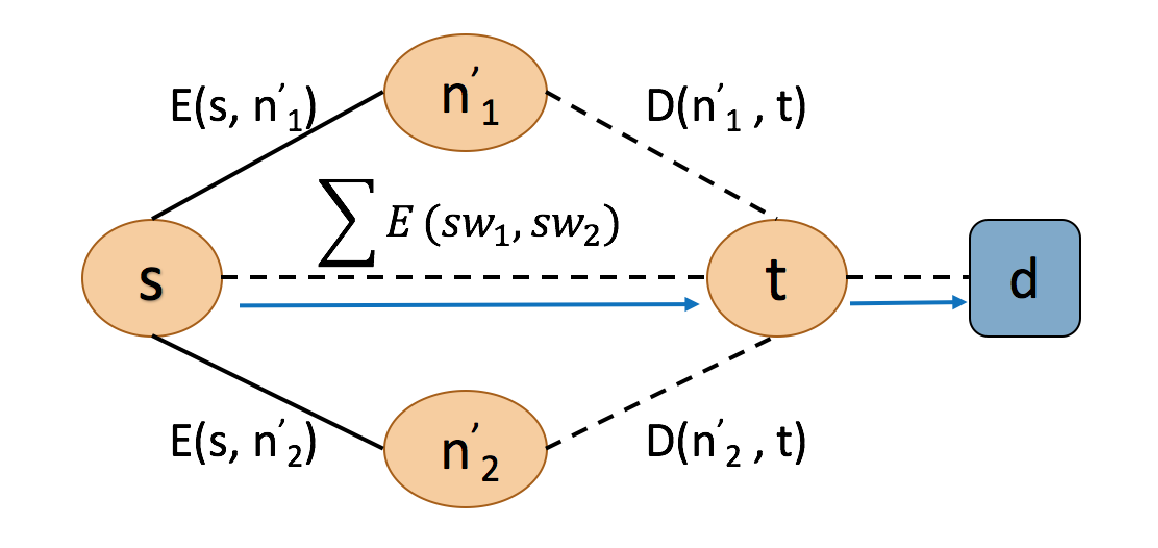
\includegraphics[width=0.8\columnwidth]{figures/distanceEquation.eps}
	\caption{An example illustration of the distance equations for shortest path forwarding.
		The pointed arrows represent the path in DAG of destination $d$, and the
		dotted line represents 1 or more edges. 
	} \label{fig:disteq}
\end{figure}
Consider a DAG $\xi_d$ for destination $d$. We define two neighbour
functions: $N_T(s)$ denotes the set of neighbours of switch $s$ 
in the input graph $T$, and $N_{\xi_d}(s)$ denote the set of
neighbours of switch $s$ in the destination DAG $\xi_d$. 
Given a destination $d\in \Omega$,
we use the following equations to ensure that, given two nodes $s$ and $t$ in
$\xi_d$, 
the set of paths from $s$ to $t$ in $\xi_d$ are
exactly
\emph{the} shortest paths from $s$ to $t$ in $T$ (\Cref{fig:disteq} illustrates 
an example).
Let $s,t$ be two nodes in $\xi_d$ and let  $Paths_{\xi_d}(s,t)$ be the set of paths from $s$ to $t$ in $\xi_d$.
\begin{multline} \label{eq:uniq1}
		\forall l_0\cdots l_n\in Paths_{\xi_d}(s,t).
		\forall n' \in N(s) \setminus N_{\xi_d}(s). \\
		E(s, n') + D(n', t) > \sum_{\mathclap{\substack{l_i=(s_i,t_i)}}} 
		E(s_i, t_i) 
\end{multline}
\begin{multline} \label{eq:uniq2}
		\forall l_0\cdots l_n\in Paths_{\xi_d}(s,t).
		\forall n' \in N_{\xi_d}(s). n' \not\rightarrow^+_{\xi_d} t.  \\
		E(s, n') + D(n', t) > \sum_{\mathclap{\substack{l_i=(s_i,t_i)}}} 
		E(s_i, t_i) 
\end{multline}
\begin{multline} \label{eq:uniq3}
		\forall l_0\cdots l_n, l_0'\cdots l_n'\in Paths_{\xi_d}(s,t).\\
		\sum_{\mathclap{\substack{l_i=(s_i,t_i)}}} 
		E(s_i, t_i)  =\sum_{\mathclap{\substack{l_i'=(s_i',t_i')}}} 
		E(s_i', t_i') 
\end{multline}
Equation~\ref{eq:uniq1} guarantees that 
the sum of the weights belonging to a path from $s$ to $t$ in $\xi_d$ is smaller than 
any path that goes to $t$ via a node $n'$ that is a neighbour of $s$ in $T$ but not in $\xi_d$.
Equation~\ref{eq:uniq2} guarantees that
the sum of the weights belonging to a path from $s$ to $t$ in $\xi_d$ is smaller than 
any path that goes to $t$ via a node $n'$ that is a neighbour of $s$ in $\xi_d$ but such that
$t$ is not reachable from $n'$ in $\xi_d$.
Finally, Equation~\ref{eq:uniq2} guarantees that all the paths from $s$ to $t$ in $\xi_d$ have the same weight.

% If the path $n' \rightarrow^* t$ 
% is not in any DAG completely, then
% $D(n',t)$ can be smaller than the actual shortest distance by the
% semantics of \Cref{eq:dist} (as
% $D(n',t)$ is not equal to any quantity by \Cref{eq:shortest}).
% However, since $D(n',t)$ is on the RHS of the equations in \Cref{eq:uniq},
% the equations will ensure that the path $s\rightarrow n \rightarrow^* t$
% has strictly greater weight than the path of the DAG.

%TODO: Add some figures

\subsubsection{Synthesis of ARC with route-filters} \label{sec:routefilter}
\begin{figure}
	\centering
	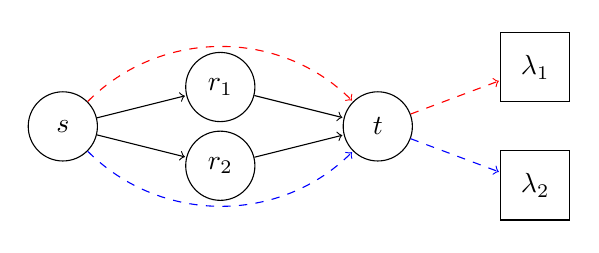
\begin{tikzpicture}[shorten >=0.5pt,node distance=,on grid,auto,
	square/.style={regular polygon,regular polygon sides=4}] 
	\node[state] at (0,0) (s)  {$s$}; 
	\node[state] at (2,0.5) (v1)  {$r_1$}; 
	\node[state] at (2,-0.5) (u1) {$r_2$}; 
	\node[state] at (4, 0)(t) {$t$};
	\node[state, rectangle] at (6, -0.75) (d2) {$\lambda_2$};
	\node[state, rectangle] at (6, 0.75) (d1) {$\lambda_1$};
	\path[->] 
	(s) edge  node {} (v1)
	edge  node {} (u1)
	edge [blue, dashed, bend right=45] node {} (t)
	edge [red, dashed, bend left=45] node {} (t)
	(u1) edge node {} (t)
	(v1) edge node {} (t)
	(t) edge [red, dashed] node {} (d1) 
	edge [blue, dashed] node {} (d2);
	\end{tikzpicture}
	\caption{Example of paths which require route-filtering. This is a
		diamond starting at $s$ and ending at $t$. The diamond can be
		eliminated by filters $((s,r_1),\lambda_2)$ or $((s,r_2),\lambda_1)$.}
	\label{fig:diamond}
\end{figure}

The sARC synthesis problem does not always admit a solution.
This blocking mechanism supported by (non-simplified)
ARC is called a route-filter. 
A route-filter  can selectively disable an
edge for a given destination by  blocking advertisements to a
particular destination along a link. 
Formally, a route-filter is a pair $(l,d)\in L\times S$
disabling a link $l$ for destination $d$
and path to a destination $d$ is \emph{unfiltered} 
if it does not contain edges that are filtered for destination $d$.
%Therefore, if a route-filter is added on switch $s3$, 
%$s3$ 
%will not advertise a route for $d1$ to $s1$, so 
%$s1$ will forward to $s2$ and not to $s3$
%to reach $d1$. The forwarding of packets destined
%for $d2$ are not affected, and they will be sent from
%$s1$ to $s4$ via $s3$ as it is the shortest path.
%Thus, by incorporating route-filters, we can
%disable certain links in the topology 
%for specific destinations, and synthesize
%ARCs for all possible data planes. 
The \emph{ARC synthesis} problem
is to find rational weights for the edges in $L$
and a set of route-filters $F\subseteq L\times S$
 such that 
for each pair of endpoints $(s,t) \in \Gamma$, 
the paths in $P(s,t)$ are the shortest \emph{unfiltered} paths from $s$ to $t$ 
in the graph. 

The ARC synthesis problem admits a trivial solution in which 
route-filters are used to enforce the exact set of input paths by blocking all other possible paths.
This can be done by creating a 
route-filter $(l,d)$ for every link $l$ not in $\xi_d$. 
However, this solution may overly restrict the structure of the network.
In particular, if two nodes were connected by a single path,
a link failure would immediately result in the network becoming disconnected!
Moreover, installing so many route-filters might be costly as not all switches might
support this mechanism.

Ideally, we would like to impose further restrictions to the ARC
synthesis problem to make sure that the obtained solution
satisfy desirable connectivity or resilience properties.
In the following we informally use the word objective 
to identify a property we desire for the synthesized ARC.
Examples of objectives are minimizing the number of route-filters
or maximizing the number of edge-disjoint paths in the ARC
for each endpoint. 
Given an objective $O$, the \emph{augmented ARC synthesis} problem
is to find rational weights for the edges in $L$
and a set of route-filters $F\subseteq L\times S$
 such that 
1) for each pair of endpoints $(s,t) \in \Gamma$, 
the paths in $P(s,t)$ are the shortest \emph{unfiltered} paths from $s$ to $t$ 
in the graph,
2) the resulting ARC satisfies the objective $O$. 
In the following we only allow route-filters for a destination $d$ to be applied to edges of $T$ that are directly connected to 
nodes in $\xi_d$. 

We propose an iterative approach to this problem. 
Our algorithm starts by trying to synthesize a solution
that does not use route-filters using the equations proposed in \secref{sec:sarc}. 
In the case of a failure, the algorithm uses the ``proof of unsatisfiability'' generated by the constraint solver 
to greedily add a small set of route-filters. New equations are then generated and approach is repeated until a solution is found.
We first describe the 
modified linear equations generated when a set of
route-filters are enabled, and then describe two
techniques used to choose route-filters. 
%\begin{figure}
%	\centering
%	\includegraphics[width=\columnwidth]{figures/arcSynthesis.eps}
%	\caption{Synthesis of ARC with route-filters.} \label{fig:arcSynthesis}
%\end{figure}

\minisection{Equations with route-filters}
We show how the technique used to solve the simplified synthesis
problem can be modified to handle filtered and unfiltered paths.
We assume we are given a set of route-filters $F$ and 
use $s\rightarrow_d^* t$ to denote that $s$ can reach $t$
in $T$ without using any edge $l$, such that $(l,d)\in F$.
We use $D_d(r_1, r_2)$ to denote the shortest distance from $r_1$ to $r_2$
using only edges that are not filtered for destination $d$.
We can revise the equation in \eqref{eq:dist} to correctly restrict the values of $D_d$
by simply ignoring all the filtered edges. 
In the same way, we can modify equations  \eqref{eq:uniq1} and \eqref{eq:uniq2}, while
equation \eqref{eq:uniq3} remains unchanged.

Unfortunately, if the encoding without route-filters produces $n$ equations, this encoding produces $|\Omega|n$ due
to the multiple different distances $D_d$.
Notice that, the shortest distance $D_d(s,t)$ between two nodes $s$ and $t$ without using edges filtered for $d$ cannot be
smaller than the shortest distance $D(s,t)$ obtained without considering route-filters.
We use this property to simplify the encoding by only computing $D(s,t)$ and by replacing each instance of $D_d(s,t)$
with $D(s,t)$ in
equations \eqref{eq:uniq1} and \eqref{eq:uniq2}. 
It is easy to see that every solution of this simplified set of constraints
is also a solution to the original solution (because $D(s,t)\leq D_d(s,t)$).
However, the reverse is not true and the set of simplified equations can be unsatisfiable
in cases in which the original set is satisfiable.
We use the simplified
set of equations in our preliminary implementation and show how it yields encouraging results in practice.

If the set of linear equations does not admit a solution, we 
can add new route-filters so that the equations resulting from the added
route-filters admit a solution.
We discuss two schemes used to add route-filters:
the first scheme uses unsatisfiable cores generated
by the solver and the second scheme 
finds geometrical structures called diamonds that 
cannot be handled without route-filters.


% While detecting diamonds is efficient, the
% presence of diamonds is a not 
% necessary condition for route-filtering.
% Characterising the properties of data planes for which there is
% a pure ARC solution (i.e., no route-filters
% required) is a open algorithmic
% problem. An 
% efficient algorithm to find the structures causing 
% inconsistencies based on these properties 
% can be used to minimize the number of route-filters enabled.  

\todo{Not good, improve} \\
\minisection{Adding filters using unsatisfiable cores}
Modern LP-solvers have efficient procedures to return an
unsatisfiable core, also called IIS (Irreducible Inconsistent Subsystem)
~\cite{chinneck2007feasibility}. Formally, an IIS is a subset of constraints such that,
if all constraints except those in the IIS are removed, the resulting set of
linear equations is still inconsistent (unsatisfiable). Moreover, the set is irreducible---i.e., removing 
any one constraint of the IIS produces a consistent set of constraints. 

Suppose that, upon producing our set of linear equations, the solver returns unsatisfiable and produces
a concrete unsatisfiable core. 
Some of the linear inequalities from 
Equations \eqref{eq:uniq1} and  \eqref{eq:uniq2}
will appear in the unsat-core 
(an unsat-core cannot consist of only 
constraints from \Cref{eq:dist} and \eqref{eq:uniq3}, as all distances and edges set to zero
would trivially be consistent with these constraints). 
In particular, the unsat-core contains some constraint
\begin{eqnarray}
E(s, n') + D(n', t) > \sum_{\mathclap{\substack{l_i=(s_i,t_i)}}} 
		E(s_i, t_i) 
\end{eqnarray}
that was added to reason about some DAG $\xi_d$.

By adding the route-filter $((s,n'),d)$ to $F$, this inequality is removed from the set of constraints
and the combination of the other constraints appearing in the other unsat-core is now satisfiable.
The complete set of equations may still be inconsistent as other unsat-cores might exist. 
The procedure can be repeated until the resulting set of constraints becomes satisfiable
and we have therefore reached a solution to the ARC synthesis problem.

Finding the optimal number of route-filters is NP-hard, and it
is very difficult to incorporate optimality in our iterative learning
technique for finding the set of filters. This is because we do not 
have the set of all unsatisfiable cores (the solver returns one at 
a time) to find an optimal set of filters. Instead of considering the 
number of filters, we consider the metric: loss of resilience.
%\loris{not sure the next paragraph is needed}
%For a given unsat-core, there may be multiple ways to place a route
%filter to eliminate one constraint and we have not investigated
%We can 
%adopt a greedy approach (based on set cover \cite{setcover}) 
%of picking a route-filter which 
%eliminates the maximum number of unsat-cores. However, 
%finding the number of unsat-cores a route-filter eliminates
%is an open problem and instrumental in minimizing the number 
%of route-filters. Other schemes can be used to choose 
%a route-filter from an unsat-core satisfying certain
%objectives. 

Finding an IIS is an NP-hard problem~\cite{iiscomplexity}
and can result in slow synthesis times.
%We identify a topological property of the set of input paths that 
%is guaranteed to require route-filters and use it to produce an initial set of necessary route-filters.
%This technique allows us to reduce the number of times we are required to compute  unsat-cores.
%
%We define the structure shown in \Cref{fig:diamond}
%as a \emph{diamond}. 
%Formally, a problem instance contains a diamond iff there exists two different destinations $d$ and $d'$
%such that, in their corresponding DAGs $\xi_d$ and $\xi_{d'}$,
%there exists two nodes $s$ and $t$, such that $s\rightarrow_{\xi_d} t$,
%$s\rightarrow_{\xi_{d'}} t$, and
%there exists a path $l_0\cdots l_n$ from $s$ to $t$ in $\xi_d$ that is not a path from
%$s$ to $t$ in $\xi_{d'}$.
%As we mentioned at the beginning, synthesizing an ARC for  diamond structures requires
%the addition of a route-filter.
%In fact, each such a diamond can be ``removed'' by introducing a route-filter $(l_0, d')$ that hides
%the path $l_0\cdots l_n$ for the destination $d'$ (see \Cref{fig:diamond}).
%Diamonds can detected and removed in polynomial time.
%%Consider
%the diamond in \Cref{fig:diamond}. There are two choices
%of route-filters: the $s1-s3$ edge for destination $d1$ 
%and the $s1-s2$ edge for destination $d2$, out of which,
%at least one filter is required to eliminate the 
%inconsistency in the linear equations caused due to the diamond.
%Thus, we find all diamonds for all pairs of destination
%DAGs (this is done in polynomial time) and assign a filter
%to one of the two edges at the source of each diamond. 
%Thus, by removing the diamonds, we can reduce the 
%number of iterations
%of the unsat-core learning approach, which would have 
%provided diamonds as an unsat-core if 
%diamonds were not eliminated.





\section{Complexity}
\begin{theorem}
Finding the set of route-filters $R$ of smallest size such
 that there exists OSPF edge weights $W$ for topology $G=(V,E)$ 
 and the resulting configurations forward traffic along the
input paths $P$ under non-failure scenarios is NP-hard.
\end{theorem}

\begin{proof}
We prove the above theorem by reducing the \emph{minimum vertex cover} problem
to finding the smallest set of route-filters and OSPF weights 
which forward traffic along the
input paths under non-failure scenarios. 

Given a graph $G_{vc}=(V_{vc},E_{vc})$ and $VC$ denotes the minimum 
vertex cover of the graph $G_{vc}$. 

\begin{lemma}
	For a 
\end{lemma}
\end{proof}
\section{Configuration Requirements}
We consider synthesis of inter-domain 
(for lack of a better word) routing 
configurations where each domain uses a 
IGP for intra-domain routing (like 
OSPF) and domains communicate among 
themselves using BGP. 
Routing inside a domain is controlled 
by synthesizing OSPF edge weights and 
route-filters. BGP is a path-vector
protocol and primarily selects routes by 
AS-PATH length. However, we can 
use BGP's powerful path selection metrics 
like local preferences to select 
paths with greater path lengths (local
preference value is considered first in 
path selection with multiple routes). 
OSPF has better convergence times than BGP,
thus, it is advantageous to use OSPF for 
routing in small domains and using BGP for
inter-domain routing. 

We introduce a framework of synthesizing
inter-domain configurations under certain
constraints. For example, due to scalability
concerns, OSPF domains must be smaller than 
a certain threshold for effective operations.
Similarily, the number of local preferences 
stored on a router is limited due to 
resource constraints. Thus, the routing 
configurations generated must adhere to 
these constraints. We describe the constraints
supported by the framework, points 1-4 are 
hard constraints we would ensure, while 5-8
are optimizations to synthesize better inter-domain
configurations. 

\begin{enumerate}
	\item \textbf{Number of domains ($N(D)$)}: 
	Can be used for administrative constraints 
	(each domain can be managed by different
	entities). 
	\begin{equation}
	N_l \leq N(D) \leq N_u
	\end{equation}

	\item \textbf{Size of domain ($|D|$)}: OSPF
	performs poorly as size of the domain increases
	(due to flooding of link-state updates). Thus,
	operators can specify bounds on the size of each
	domain.
	\begin{equation}
	S_l \leq |D| \leq S_u
	\end{equation}

%	\item \textbf{BGP-Compatibility}: Certain 
%	routers may not be suited to run BGP due to resource
%	constraints. Thus, the operator can specify if a 
%	router is non-BGP compatible. 

	\item \textbf{Optimization: Lines of configuration} 
	To enable path-based inter-domain routing, \name needs
	to set up static routes along the path, or configure BGP 
	variables like local preferences to 
	to ensure the routing emulates the input paths under no 
	failures. This would increase the size of the configurations,
	thus increasing the complexity of verifying correctness either 
	manually or using verification tools~\cite{batfish}. 

\end{enumerate}

\section{MCMC Sampling}
\name tackle the problem of minimization of LoC/route-filters
by stochastically searching for a domain assignment which 
minimizes the cost of the configuration with the help of Markov
Chain Monte Carlo (MCMC) sampling, specifically the Metropolis-Hasting
algorithm, a common technique used in different optimization 
problems~\cite{stoke}. 

MCMC sampling is a technique for drawing elements from a
probability density function in direct proportion to its value: re-
gions of higher probability are sampled from more often than 
regions of low probability.
Applied in cost minimization problems,
MCMC sampling acts as an intelligent hill climbing method which
is robust for irregular cost functions and avoids convergence at 
local minimas. To transform an arbitrary cost function $c(\Theta)$, 
into a probability density function, we use the following 
technique~\cite{mcmcbook}:
\begin{equation}
	p(\Theta) = \frac{1}{Z}exp(-\beta * c(\Theta))
\end{equation}
$\beta$ is a positive constant and $Z$ is a partition function that
normalizes the distribution. Computing $Z$ is in general 
intractable, and the Metropolis-Hasting algorithm for 
generating Markov Chains can explore the probability density
function $p(\Theta)$ without computing the partition function. 
The intuition is as follows: given a current domain
assignment $\Theta$, the algorithm proposes a modified 
domain assignment $\Theta'$ as the next step. $\Theta'$
is accepted or rejected based on the Metropolis-Hasting
acceptance probability: 
\begin{equation}
Pr(\Theta \rightarrow \Theta') = min(1, \frac{p(\Theta')*q(\Theta| \Theta')}{p(\Theta)*q(\Theta'| \Theta)})
\end{equation}
$q(\Theta'| \Theta)$ denotes the proposal distribution from 
which $\Theta'$ is chosen given $\Theta$. If the proposal 
distributions is symmetric, i.e., 
$q(\Theta| \Theta') = q(\Theta'| \Theta)$, then the acceptance
probability is reduced to the simpler Metropolis ratio, which
can be computed directly from the cost function $c(\Theta)$:
\begin{multline}
Pr(\Theta \rightarrow \Theta') = min(1, \frac{p(\Theta')}{p(\Theta)}) \\
= min(1, exp(-\beta.(C(\Theta') - C(\Theta)))
\end{multline}
As we can observe from the acceptance probability, 
the algorithm will always accept a new proposal $\Theta'$
if its cost is lower than $\Theta$. If $\Theta'$ has a 
higher score than $\Theta$, the proposal will be 
probabilistically accepted depending on 
how far the cost of the proposals are. This ensures that 
the algorithm does not get stuck at local minimas and 
explore proposals with smaller differences in cost with 
higher probability. We describe the MCMC search procedure 
in Pseudocode~\cref{alg:mcmc}. 

\subsection{Hard Constraints}
\begin{algorithm}[t]
	\floatname{algorithm}{Pseudocode}
	\caption{MCMC}
	\label{dcsyn}
	\begin{algorithmic}[1] \label{alg:mcmc}
		\Procedure{MCMCSearch}{}
		\State{$\Theta \leftarrow$ random domain assignment}
		\State{$\overline{cf} = 0$ \hspace{2cm} [Worst Conf. overhead]}
		\State{$\overline{rf} = 0$ \hspace{2cm} [Worst route-filter est.]}
		\While{max iterations OR timeout}
		\State{$\gamma$ = \Call{Cost}{$\Theta$}}
		\State{$\Theta'$ = \Call{RandomChange}{$\Theta$}}
		\State{$\gamma'$ = \Call{Cost}{$\Theta'$}}
		\State{$Pr(\Theta \rightarrow \Theta')$ = 
			min$(1, exp(-\beta.(\gamma' - \gamma))$}
		\State{Set $\Theta$ = $\Theta'$ with 
			probability $Pr(\Theta \rightarrow \Theta')$}
		\EndWhile
		\EndProcedure
		
		\Procedure{Cost}{$\Theta$} 
		\State{$cf \leftarrow$ Configuration overhead (Static routes + \newline \hspace*{1.5cm} 
			BGP local preference entries + iBGP filters)}
		\If{$cf > \overline{cf}$} 
		\State{$\overline{cf} = cf$}
		\EndIf
		\State{$rf \leftarrow$ Number of diamonds with  \newline 
			\hspace*{1.3cm}  endpoints in same domain }
		\If{$rf > \overline{rf}$} 
		\State{$\overline{rf} = rf$}
		\EndIf
		\State{$\gamma$ = max($cf/\overline{cf},
			\alpha.rf/\overline{rf}$)  \newline
			\hspace*{3.5cm} + 0.1*min($cf/\overline{cf},
			\alpha.rf/\overline{rf}$)}
		\State{\Return $\gamma$}
		\EndProcedure
		
		\Procedure{RandomChange}{$\Theta$}
		\While{True}
		\State{$r \leftarrow$ pick random boundary router}
		\State{$\theta \leftarrow$ pick random neighbouring domain of $r$}
		\If{$|\Theta(r)| - 1 \geq l_\Theta \wedge |\theta| + 1 \leq u_\Theta$}
		\State{$\Theta' \leftarrow \Theta[r \rightarrow \theta]$} \hfill [$r$'s domain changed to $\theta$]
		\If{domains are continous}
		\State{\Return $\Theta'$}
		\EndIf
		\EndIf
		\EndWhile
		\EndProcedure
	\end{algorithmic}
	
\end{algorithm}

\subsection{Configuration Cost}
\todo{Explain path, as\_path transformation more formally}
\subsubsection{Static Routes} \label{sec:static}
As shown in \Cref{} (Refer to example of 
static routes in motivating example), we require static routes 
to enforce AS paths with loops. Static routes have the lowest 
administrative distance (1) by default~\cite{ad}, and will override BGP
and OSPF routes at a router, this feature can be used to 
exit and enter a domain multiple times. While static routes
do not reduce the resilience of the network (all routes are still
enabled, unlike route-filters), a network under flux will have
unpredictable routing behaviour, unlike with only OSPF and BGP
configured at the routers. 
Also, static routes have to be installed per-destination, thus increasing
the size of configurations drastically as number of policy paths increase.

Given a path $p$ for subnet $\lambda$ and 
the corresponding AS path $p_{as}
= as_1 \rightarrow as_2 \rightarrow \ldots \rightarrow as_m$ (where
$as_m = \Theta(\lambda)$), static
routes are required if $p_{as}$ has a AS-loop. 
To minimize
the number of static routes, we find 
the smallest $i \in [1,m]$ 
such that $\overline{p_{as}} = as_i \rightarrow as_{i+1}
\rightarrow \ldots \rightarrow as_m$ has no loops. 
Therefore, $\overline{p_{as}}$ is the longest AS-loop-free
subpath of $p_{as}$, and be can be enforced using BGP and OSPF. For the 
network path corresponding to AS path $as_1 \rightarrow as_2 
\rightarrow \ldots \rightarrow as_{i-1}$, we require static
routing rules for each next-hop. The static routing score
is the total number of static route hops required to enforce
the input paths.
\todo{Write about the BGP paths are extracted for the next phase}

\subsubsection{BGP Local Preference Entries}
\name uses BGP local preference to route traffic
for a particular subnet to the next AS via a specific 
gateway as per the input paths obtained. 
As shown in \Cref{} (Refer
to ex), if there are multiple exit gateways from an AS 
for a subnet $\lambda$, we require local preference entries at the 
gateways and iBGP filters among these gateways for $\lambda$.

For a domain $d$ and subnet $\lambda$, consider the set 
of paths to $\lambda$ exiting $d$ using BGP (and not statically
routed as described in \Cref{sec:static}). Let $E$ denote the
set of exit gateway routers for the paths of $\lambda$. 
If $|E| = 1$, if gateway $g \in E$ receives a route with 
strictly shortest AS path length (\Cref{alg:bgppathrules}) 
which enforces the paths
for $\lambda$, we do not need to configure local preference
entries on any BGP router in the domain for $\lambda$. If
the exit route chosen by the gateways for $\lambda$ does not 
enforce the paths, \name configures a local preference entry
for $\lambda$ at exit gateway, and thus, the exit route chosen
by BGP enforces the input paths for $\lambda$ in the domain.

If $|E| ~> 1$, multiple BGP routes must be redistributed to 
the OSPF domain. \\
E local prefs + E(E - 1) iBGP filters!

\todo{Changes to OSPF synthesis to ensure closest gateway}

\subsection{Route-Filter Cost}










\begin{figure}[t]
	\centering
	\includegraphics[width=0.7\columnwidth]{figures/ospfSynthesisTimeMCMC.eps}
	\compactcaption{MCMC OSPF Synthesis time}
	\label{fig:ospfmcmc}
\end{figure}


\begin{figure}[t]
	\centering
	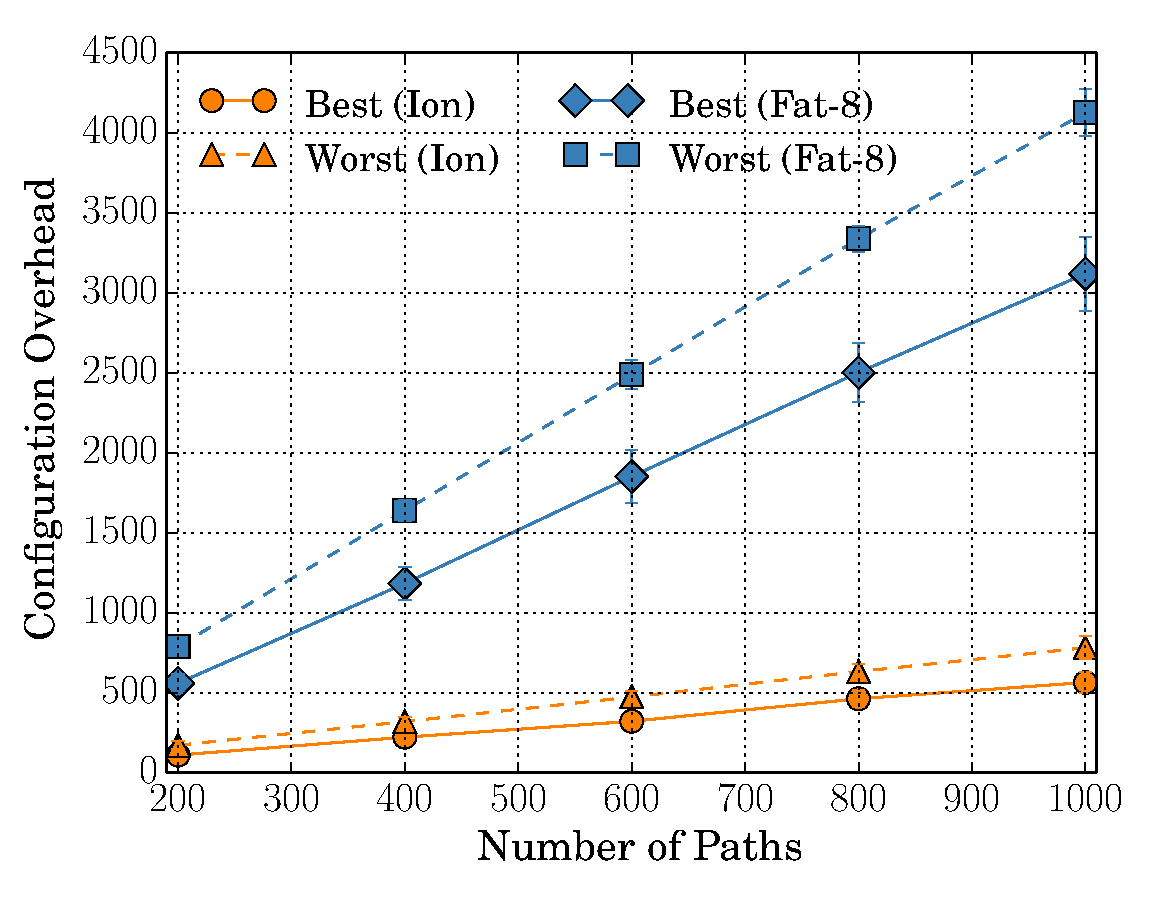
\includegraphics[width=0.7\columnwidth]{figures/confMCMC.eps}
	\compactcaption{MCMC Lines of Conf}
	\label{fig:confmcmc}
\end{figure}

\begin{figure}[t]
	\centering
	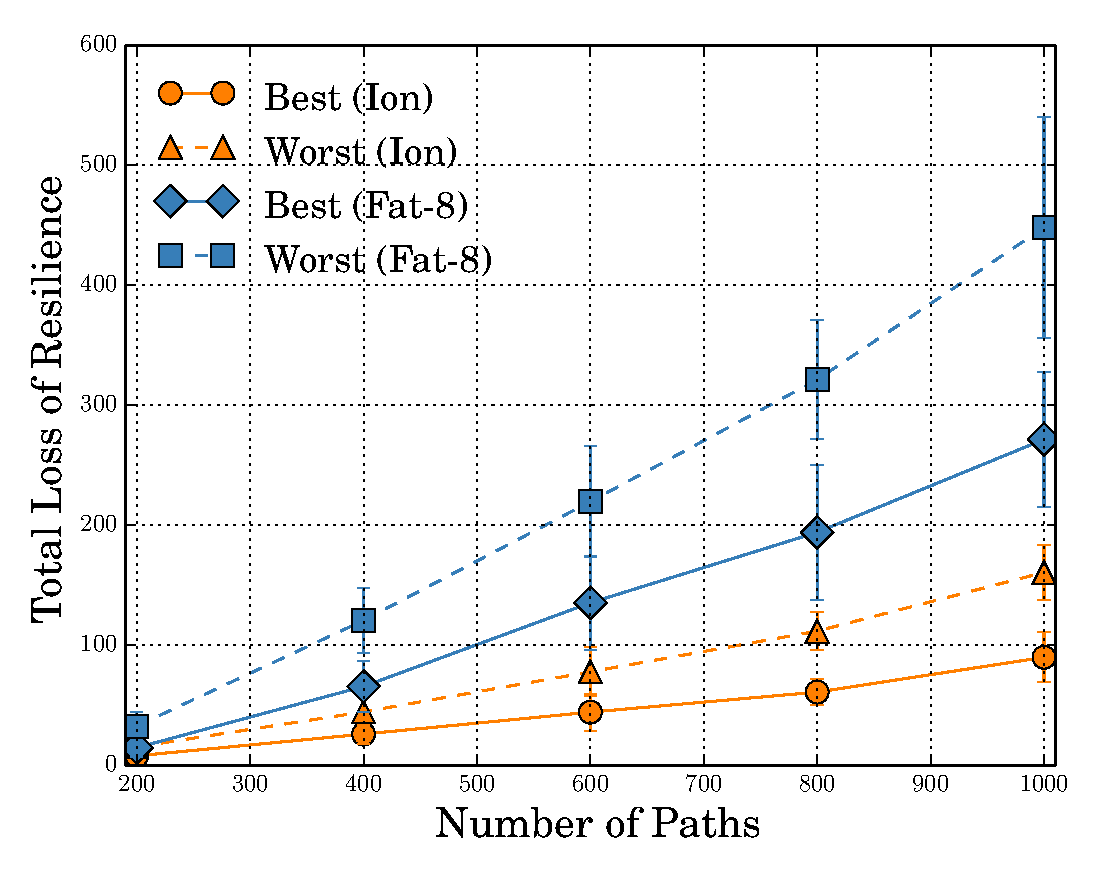
\includegraphics[width=0.7\columnwidth]{figures/TRLMCMC.eps}
	\compactcaption{MCMC TRL}
	\label{fig:trlmcmc}
\end{figure}



\section{Evaluation}
%\category{CR-number}{subcategory}{third-level}
%
%% general terms are not compulsory anymore,
%% you may leave them out
%\terms
%term1, term2
%
%\keywords
%keyword1, keyword2


%\acks
%
%Acknowledgments, if needed.

% We recommend abbrvnat bibliography style.

\bibliographystyle{abbrvnat}

% The bibliography should be embedded for final submission.
\bibliography{references}
\iffull
 \appendix
 
\section{NP-completeness Proof of Enforcing Isolation Policies} \label{sec:isolationNP}
 We show that the graph 3-coloring problem, which is NP-complete reduces to the enforcement problem for
 reachability and isolation policies. The latter is also in NP, so after the reduction we 
 can conclude that it is also NP-complete.

Let $G=(V,E)$ be an instance of the graph 3-coloring problem.
The graph $G$ admits a 3-coloring if there exists a function 
$f:G\mapsto \{R,G,B\}$ such that for every edge $(v1,v2)\in E$,
$f(v_1)\neq f(v_2)$.

We now show how to construct a topology $T=(S,L)$ and a corresponding set of policies $P$ that can be 
enforced iff $G$ admits 3-coloring.
The topology $T$ is the one depicted in  \Cref{fig:swtopo}.
The set of flows is $V$, $v \in V$ we add a reachability policy $s >> d$ on the flow $v$.
For each edge $(v1,v2)\in E$ we add an isolation policy $v_1||v_2$.
% \begin{figure}[H] 
% 	\centering
% 	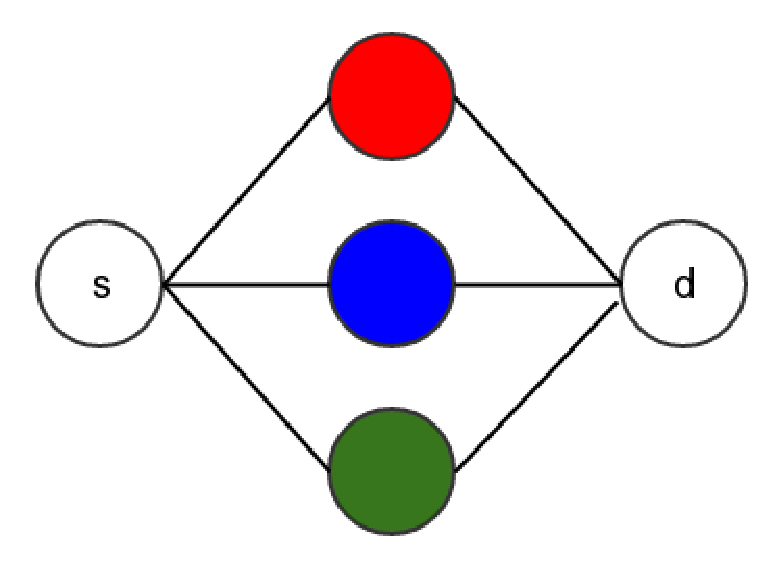
\includegraphics[width=0.5\columnwidth]{figures/color_topo.eps}
% 	\caption{The switch topology $T$. All circles represent switches and all reachability policies are $s$ to $d$}
% 	\label{fig:swtopo}
% \end{figure}
\begin{figure}[h!]
	\centering
	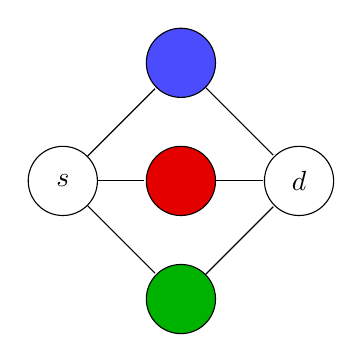
\begin{tikzpicture}[shorten >=0.5pt,node distance=1.5cm,on grid,auto] 
	\node[state] (s)   {$s$}; 
	\node[state, fill=black!10!red] (r) [right=of s] {}; 
	\node[state, fill=white!30!blue] (b) [above=of r] {};
	\node[state, fill=black!30!green] (g) [below=of r] {}; 
	\node[state] (d) [right=of r] {$d$}; 	
	\path[-] 
	(s) edge  node {} (r)
	edge node {} (b)
	edge node {} (g)
	(r) edge node {} (d)
	(g) edge node {} (d)
	(b) edge node {} (d);
	\end{tikzpicture}
	\caption{The switch topology $T$. All circles represent switches and all reachability policies are $s$ to $d$}
	\label{fig:swtopo}
\end{figure}
We now prove that if the policies can enforced then $G$ admits 3-coloring.
If the policy is enforced, we have a path from $s$ to $d$ for each flow/vertex $v$.
We can set $f(v)$ to the color of the corresponding middle-switch being crossed.
Since for every $(v1,v2)\in E$ the two flows for $v_1$ and $v_2$ cannot share any edge,
they must have crossed two middle-switches with different colors and $f$ is a correct 3-coloring.
The other direction of the proof is analogous.

 
% \subsection{Enforcement of Waypoint Policies}
% Given a undirected graph $G={V,E}$. Let us assume there exists an polynomial-time algorithm to compute the reachability paths satisfying the policies of the following types on the graph : \\
% \begin{itemize} 
% 	\item \textbf{P1} : $v_1 >> v_2 \Rightarrow$ There exists a path from $v_1$ to $v_2$ satisfying all input policies. A property of the path is that it does not have repeat a vertex (no forwarding loops).
% 	\item \textbf{P2} : $v_1 >> W >> v_2 \Rightarrow$ The path from $v_1$ to $v_2$  should pass through the vertices in the set $W$ in any order, without repeating a vertex.
% \end{itemize}
% \textbf{Reduction of Hamiltonian Cycle Problem} : Given a undirected graph $G={V,E}$, find $v \in V$ such that the degree of $v$ is the minimum in the graph (Will work for any vertex actually). If a Hamiltonian cycle is present in the graph, it will have the vertex $v$ in the cycle, and one of the edges from $v$.  \\
% Lets take a $n \in Neighbours(v)$. Let the input policies to our algorithm be : 
% \begin{itemize}
% 	\item \textbf{P4} : $v >> W >> n$ where $W = V - \{v,n\} $ 
% \end{itemize}
%P4 cimputes a simple path from $v$ to $n$ which passes through all the other vertices in the graph which is the Hamiltonian path problem. Since computing the Hamiltonian path is NP-hard, the problem of path computation for the waypoint policies as specified is NP-hard. 
\section{Tactics}
\begin{theorem}[Soundness]
	For a packet class $pc$, if the path $\pi \models_{pc} \Psi \wedge \Psi_R$, then $\pi \models R$.
\end{theorem}
\begin{proof}
	The proof of this theorem is by contradiction for each type of tactic. \newline
	\textbf{Type 1}: R = $\neg (l_{src} .^i .^* l_{dst})$ \\
	%$\forall sw,k \geq i + 1. (sw,pc,k) \notin Reach \implies \pi \models \neg (l_{src} .^i .^* l_{dst}) $ \newline
	\textbf{Assume  $\pi \not\models R$}.  $\pi \models l_{src} .^i .^* l_{dst}$. \\
	Thus, $\pi = src\ sw_1 \ldots sw_i \ldots dst$. \\
	Therefore,  $(dst, pc, k_{dst}) \in Reach, k_{dst} \geq i + 1$. \\
	However, $\pi \models_{pc} \Psi_R \Leftrightarrow \pi \models_{pc} \forall sw,k \geq i + 1. (sw,pc,k) \notin Reach$.
	Contradiction, as $\exists sw, k \geq i + 1. (sw,pc,k) \in Reach$.
	\newline
	\newline
	\textbf{Type 2}: $R = \neg (l_{src} .^i \ l \ .^* l_{dst})$ \newline
	\textbf{Assume  $\pi \not\models R$}. $\pi \models l_{src} .^i \ l \ .^* l_{dst}$. \\
	Thus, $\pi = src\ sw_1 \ldots sw_i \ sw_{i+1} \ldots dst$ such that $\phi(sw_{i+1}) = l$. Also $sw_{i+1} \not=dst$ (dst has to be the last switch in $\pi$)\\
	Therefore,  $(sw_{i+1}, pc, i+1) \in Reach$. \\
	However,
	$\pi \models_{pc} \Psi_R \Leftrightarrow \pi \models_{pc}\forall sw.~ \phi(sw) = l ~\wedge~ sw \not= dst \implies  (sw, pc, i + 1) \notin Reach$. \\
	Contradiction, as $\exists sw. ~ \phi(sw) = l ~\wedge~ sw \not= dst \wedge (sw,pc,i+1) \in Reach$.
	\newline \newline
	\textbf{Type 3}: $R = \neg (l_{src} .^i \ l_1 \ l_2 \ .^* l_{dst})$ \newline
	\textbf{Assume  $\pi \not\models R$}. $\pi \models l_{src} .^i \ l_1 \ l_2 \ .^* l_{dst}$. \\
	Thus, $\pi = src\ sw_1 \ldots sw_i \ sw_{i+1} \ sw_{i+2} \ldots dst$ such that $\phi(sw_{i+1}) = l_1, \phi(sw_{i+2}) = l_2$. Also $sw_{i+2} \not=dst$ (dst has to be the last switch in $\pi$)\\
	Therefore,  $(sw_{i+1}, pc, i+1) \in Reach \wedge (sw_{i+1}, sw_{i+2}, pc) \in Fwd$. \\
	However,
	$\pi \models_{pc} \Psi_R \Leftrightarrow \pi \models_{pc} \forall n_1, n_2.~\phi(n_1) = l_1~\wedge~ \phi(n_2) = l_2 ~\wedge~ n_2 \not=dst  \implies 
	\neg (Reach(n_1, pc, i + 1) \wedge Fwd(n_1, n_2, pc))$. \\
	Contradiction, as $\exists n_1. n_2. ~\phi(n_1) = l_1~\wedge~ \phi(n_2) = l_2 ~\wedge~ n_2 \not=dst \wedge Reach(n_1, pc, i + 1) \wedge Fwd(n_1, n_2, pc)$. 
\end{proof}
\begin{theorem}[Completeness]
	For a packet class $pc$, if the path $\pi \models_{pc} \Psi ~\wedge~ \pi \models R$, then $\pi \models_{pc} \Psi_R$.
\end{theorem}
\begin{proof}
	The proof of this theorem is by contradiction for each type of tactic. \newline
	\textbf{Type 1}: $R = \neg (l_{src} .^i .^* l_{dst})$ \newline
	\textbf{Assume  $\pi \not\models_{pc} \Psi_R$}. $\pi \not\models_{pc} \forall sw,k \geq i + 1. (sw,pc,k) \notin Reach$ \newline
	Therefore $\exists sw, k \geq i + 1. (sw,pc,k) \in Reach$. \\
	Therefore, $\pi \models l_{src}\ .^i \ .^* \ \phi(sw) \ .^* \ l_{dst} \implies \pi \models l_{src} .^i .^* l_{dst}$
	Contradiction, as $\pi \models R$.
	\newline 
	\newline 
	\textbf{Type 2}: $R = \neg (l_{src} .^i \ l \ .^* l_{dst})$ \newline
	\textbf{Assume  $\pi \not\models_{pc} \Psi_R$}.  $\pi \not\models_{pc}\forall sw.~ \phi(sw) = l ~\wedge~ sw \not= dst \implies  (sw, pc, i + 1) \notin Reach$. \\
	Therefore $\exists sw. \ sw \not= dst \ \wedge \ \phi(sw) = l \ \wedge \ (sw,pc,i+1) \in Reach$. \\
	Therefore, $\pi \models l_{src}\ .^i \ l \ .^* \ l_{dst}$. \\
	Contradiction, as $\pi \models R$. 
	\newline  
	\newline
	\textbf{Type 3}: $R = \neg (l_{src} .^i \ l_1 \ l_2 \ .^* l_{dst})$ \newline
	\textbf{Assume  $\pi \not\models_{pc} \Psi_R$}.  $\pi \not\models_{pc} \forall n_1, n_2.~\phi(n_1) = l_1~\wedge~ \phi(n_2) = l_2 ~\wedge~ n_2 \not=dst  \implies 
	\neg (Reach(n_1, pc, i + 1) \wedge Fwd(n_1, n_2, pc))$. 
	Therefore $\exists n_1, n_2. ~\phi(n_1) = l_1~\wedge~ \phi(n_2) = l_2 ~\wedge~ n_2 \not=dst ~\wedge~ Reach(n_1, pc, i + 1) ~\wedge~ Fwd(n_1, n_2, pc)$. \\
	Therefore, $\pi \models l_{src}\ .^i \ l_1~l_2 \ .^* \ l_{dst}$. \\
	Contradiction, as $\pi \models R$.
\end{proof}
\fi

\end{document}
